\section{Problem 7}

In this problem we’ll further analyze the data taken with the Stanford 46-meter
diameter dish. The gain of the Stanford dish is so great (about 50 dB at the GPS
L1 frequency) that you can actually see the transitions induced by the GPS L1
C/A code and by the GPS L1 P(Y) code. Recall that in lecture the GPS L1 signal
structure was presented as

\begin{equation}
	S_{L1} (t) = \sqrt{2P_{C1}} D(t) C(t) cos(2 \pi f_{L1} t + \theta_{L1} ) +
	\sqrt{2P_{Y1}} D(t) Y(t) sin(2 \pi f_{L1} t + \theta_{L1} )
\end{equation}

You can see from this that the GPS C/A code (spreading code C(t), chipping at
1.023 MHz) is in phase quadrature with the GPS Y code (spreading code Y (t),
chipping at 10.23 MHz).

Load the “Big Dish” data into your workspace in Matlab (you can use the
bigDishPSD.m script to do this). The sampling rate for these data is
$fs = 46.08 MHz$. The data are loaded into the Matlab complex variable Y. Each
element in Y represents a complex sample of the GPS signal $S_{L1}(t)$ after
mixing to baseband. The researchers who recorded the data mixed the incoming
signal to baseband with a fairly accurate estimate of the signal’s instantaneous
center frequency (including Doppler). Hence, the baseband samples have only a
small residual frequency, which gives rise to a slow rotation in the phase. If
you only look at, say, 400 samples, the phase doesn’t change much and you can
see a pattern emerge when you plot individual samples in the complex plane. (If
you look at much more than 400 samples, the slow phase rotation turns this
pattern into a donut shape.) Generate a plot similar to Fig. 1 by finding a
window of 400 samples of data within Y whose real and imaginary components form
a square that is aligned with the plot axes. Having identified such a window,
look at the real and imaginary components of Y over this window in the time
domain. Identify for your plot what signal component from SL1 (t) happens to be
in real(Y) and what component happens to be in imag(Y) over this window. Measure
the smallest chip interval for both codes. Estimate from your data the ratio of
the C/A code amplitude to the P (Y ) code amplitude.

\subsection{MATLAB code}

\begin{lstlisting}
%% Problem 6
clear all; clc; close all;
addpath("research/toolbox/")

%----- Load data
load('prn31_22apr03_01hrs40min00sec_gmt_fl1_46_08mhz_250msec.mat');

start = 8000;
Y_windowed = Y(start:start+400,:);

% Plotting the complex representation of the signal such that it forms a
% "perfect" square in the the complex plane.
figure()
plot(Y_windowed,'.')
xlabel('In phase');
ylabel('Quadrature');
title('Complex representation of the baseband signal');

t = XDelta*(0:400) * 1e6;
CA_code = real(Y_windowed);
Y_code = imag(Y_windowed);

% Plotting the real and imaginary parts of the signal
figure()
subplot(2,1,1)
    plot(t,CA_code)
    xlabel('time [us]');
    ylabel('X_{In-phase}');
    title('Time-domain representation of X_{In-phase}');

subplot(2,1,2)
    plot(t, Y_code)
    xlabel('time [us]');
    ylabel('X_{Quadrature}');
    title('Time-domain representation of X_{Quadrature}');

% The ratio of the C/A code amplitude to the P(Y) code amplitude
ratio = mean(sqrt(CA_code.^2)) / mean(sqrt(Y_code.^2)) % Amplitude of C/A_code is ~1.4x P(Y) code amplitude 
\end{lstlisting}

\subsection{Results}

Figure~\ref{fig:ex7_quadrature} shows the complex representation of the signals
in phase-quadrature.

\begin{figure}[H]
	\centering
	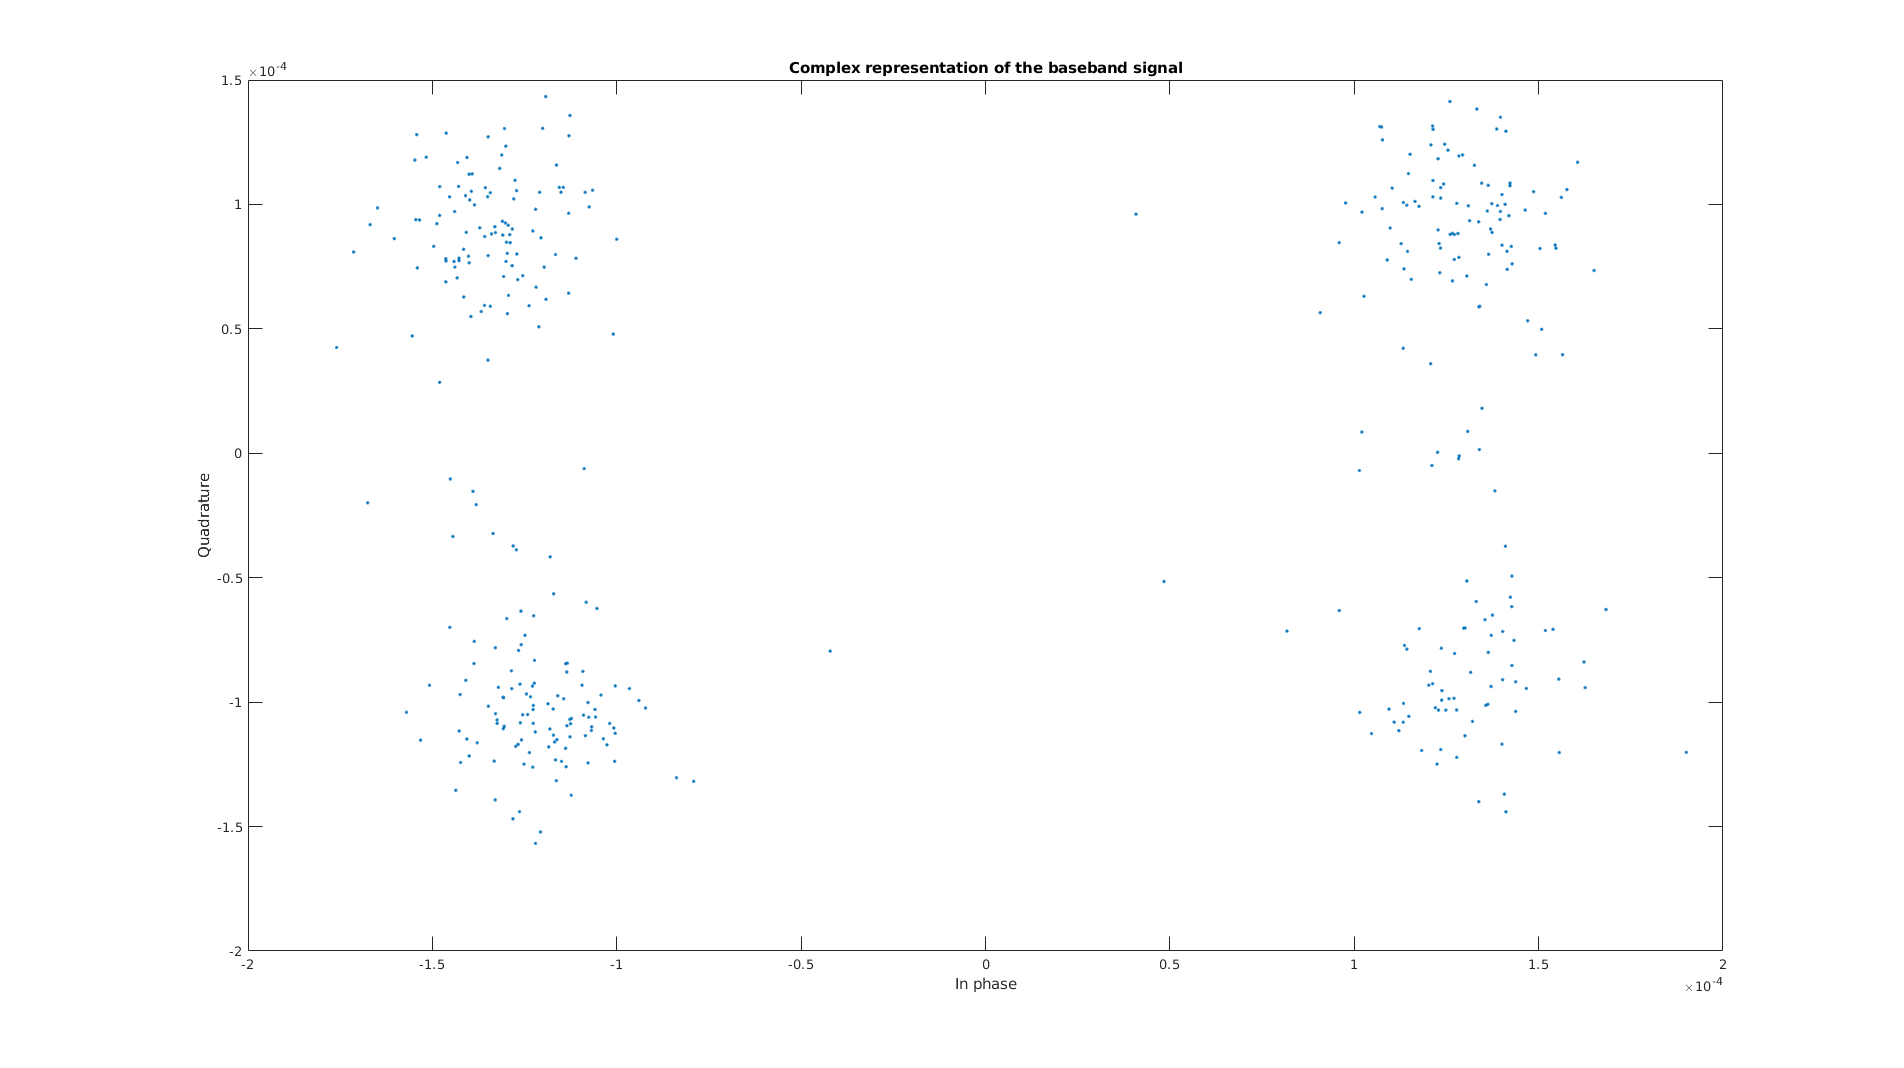
\includegraphics[width=0.9\textwidth]{figs/ex7_quadrature.png}
	\caption{Individual samples of the Stanford "Big Dish" data plotted in the
		complex plane.}
	\label{fig:ex7_quadrature}
\end{figure}

Figure~\ref{fig:ex7_time_domain}, shows the time-domain representation of the
previously shown phase-quadrature signals. It it possible to distinguish the
GPS L1 C/A-code in the top plot. It can be appreciated from the graph that the
period of the signal is $~1 \mu s$. The bottom graph exposes the P(Y)-code,
characterized by its faster chipping of $~0.1 \mu s$.

\begin{figure}[H]
	\centering
	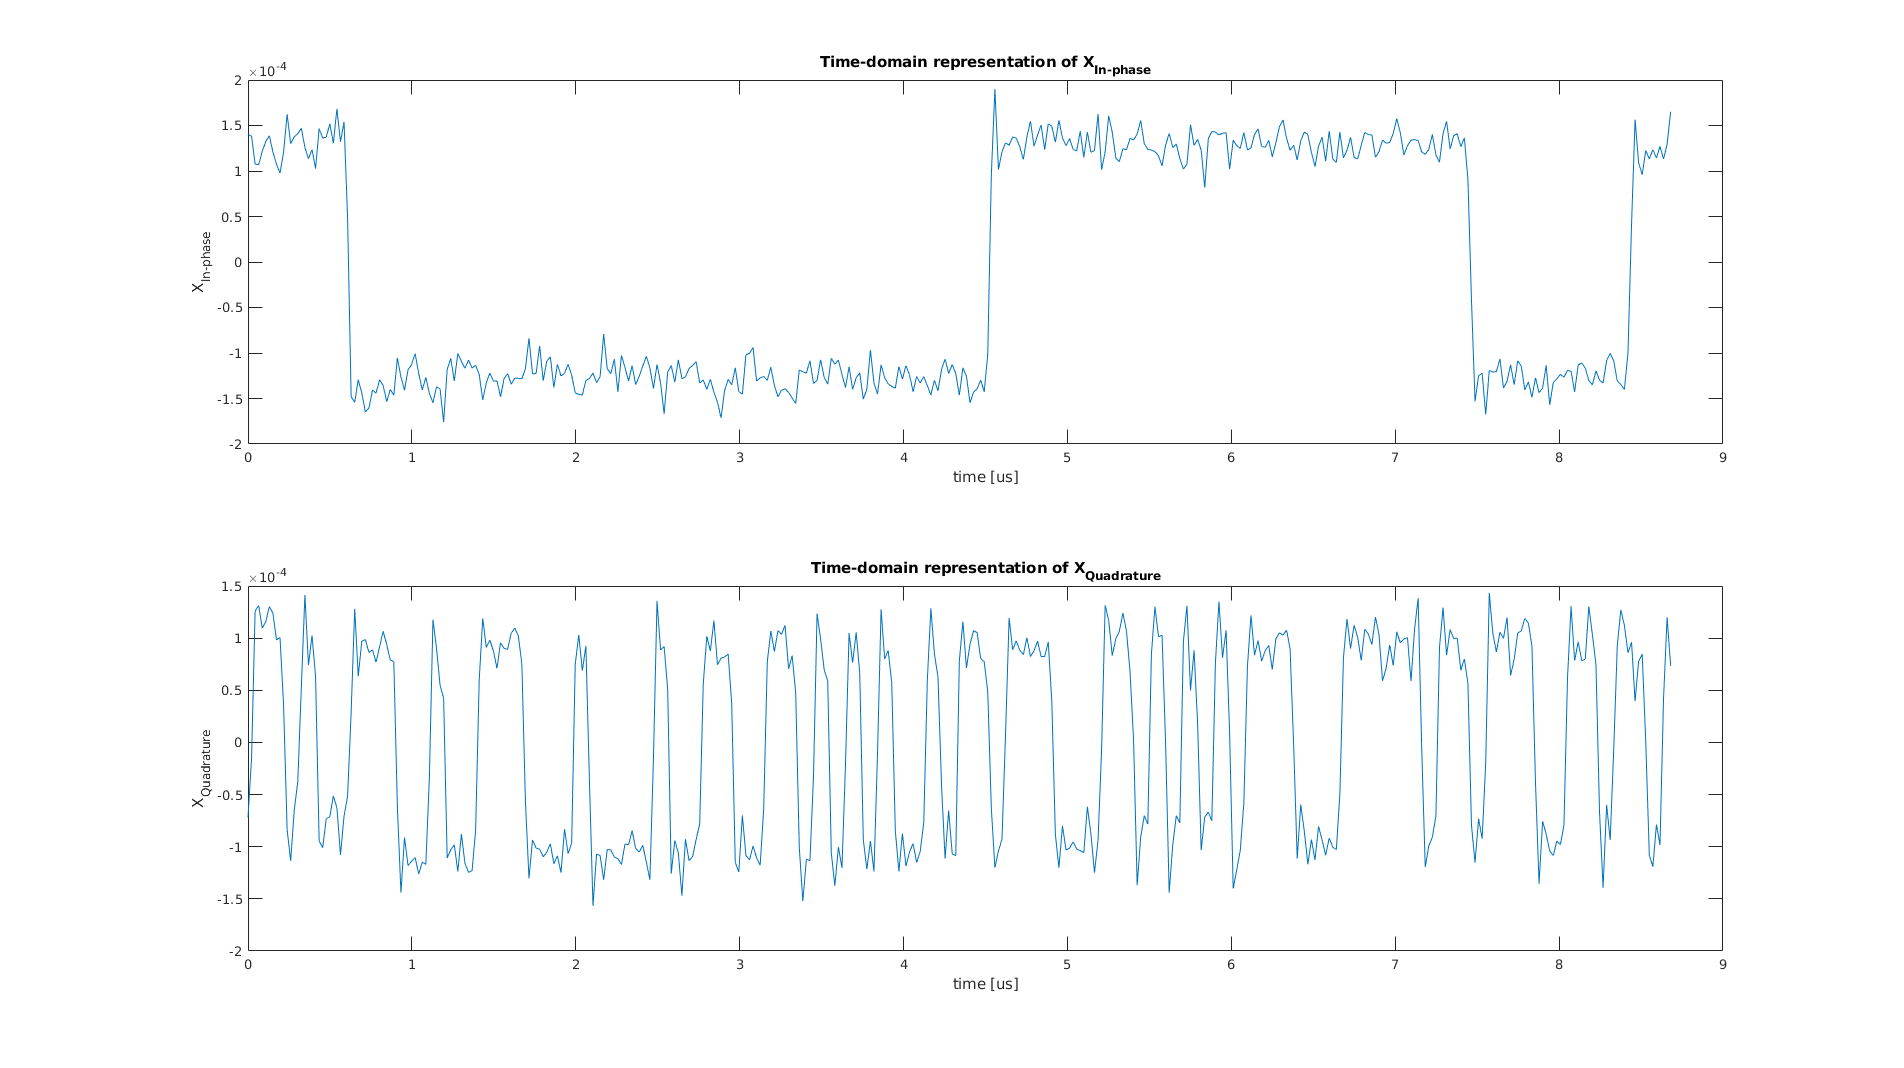
\includegraphics[width=0.9\textwidth]{figs/ex7_time_domain.png}
	\caption{Time-domain representation of the signals previously shown in
		phase-quadrature.}
	\label{fig:ex7_time_domain}
\end{figure}

Finally, the ratio of the C/A-code amplitude to the P(Y)-code amplitude reveals
that the C/A-code amplitude is $~1.4$ times larger than P(Y)-code amplitude.

